% A hound — four legs, low to the ground, in profile. The one family in the
% ladder that reads as fast rather than heavy.
%
% Written by filling in tikz_figure_prompt.md.
\documentclass[tikz,border=4pt]{standalone}
\usetikzlibrary{calc}
\providecommand{\Main}{7E8C63}
\providecommand{\Dark}{4E5940}
\providecommand{\Accent}{C4D84A}

\newcommand{\Unit}{0.055cm}
\newcommand{\Edge}{2.0pt}
\newcommand{\Legs}{4}
\newcommand{\Ridge}{5}        % spines along the back

\definecolor{main}{HTML}{\Main}
\definecolor{dark}{HTML}{\Dark}
\definecolor{accent}{HTML}{\Accent}
\definecolor{ink}{HTML}{101018}

\begin{document}
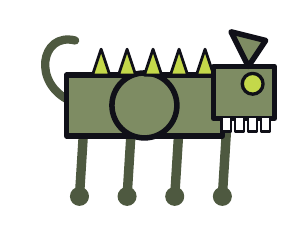
\begin{tikzpicture}[x=\Unit,y=\Unit, line join=round, line cap=round]

  % ---- legs, behind the body ----------------------------------------------
  \foreach \i in {1,...,\Legs} {
    \pgfmathsetmacro\x{14+(\i-1)*11}
    \draw[dark,line width=3.4pt] (\x,22) -- (\x-1,6);
    \fill[dark] (\x-1,6) circle (2.2);
  }

  % ---- tail ---------------------------------------------------------------
  \draw[dark,line width=3.0pt] (11,28) .. controls (2,32) and (4,44) .. (12,42);

  % ---- body ---------------------------------------------------------------
  \fill[main,draw=ink,line width=\Edge] (10,20) rectangle (46,34);
  \fill[main,draw=ink,line width=\Edge] (28,27) circle (7.5);

  % ---- the ridge, which is what makes it a hound and not a dog ------------
  \foreach \i in {1,...,\Ridge} {
    \pgfmathsetmacro\x{16+(\i-1)*6}
    \fill[accent,draw=ink,line width=1.0pt] (\x,34) -- (\x+2,40) -- (\x+4,34) -- cycle;
  }

  % ---- head ---------------------------------------------------------------
  \fill[main,draw=ink,line width=\Edge] (44,24) rectangle (58,36);
  \fill[main,draw=ink,line width=\Edge] (52,36) -- (48,44) -- (56,42) -- cycle;  % ear
  \fill[accent,draw=ink,line width=1.2pt] (53,32) circle (2.4);                  % eye
  % Teeth along the muzzle.
  \foreach \x in {46,49,52,55} {
    \fill[white,draw=ink,line width=0.8pt] (\x,21) rectangle ++(2,3.4);
  }

\end{tikzpicture}
\end{document}
